So far I have discussed the formalisation of \kl{CN}, the formalistaion and
implementation of its memory model, \kl{CN-VIP}. In both those sections,
guiding design choices and implementation decisions at each stage was the need
to strike a balance of expressiveness, performance and ergonomics,
fundamentally motivated by designing a \emph{capable} verification tool. Not
only that, at several stages, the theory was able to inform or clarify
implementation related issues, such as the complexity of adding new features,
lifting existing restrictions, or substantially improving performance.

In this part, I will take a step back and focus more on what it takes to build
a \emph{usable} verification tool. Though not as theoretically intruiging or
elegant as some of the material in the previous chapter, this is where just as
much, if not more, of the difficulty lies in achieving \kl{CN}'s goal of being
maintainable by kernel programmers (\cref{sec:cn-goals}).

It start with the source repository for any mature C project, such ask
\kl{pKVM}. It intentionally lives in the Linux kernel, indeed in many respects
this is an advantage. It is an unignorable reminder that C in the real word
however does not come neatly packaged up into isolated files of ISO grammar
conforming translations units. Aside from the myriad extensions that it relies
on, as well as non-ISO conforming C features, the inclusion chain of one file a
few hundred lines long can stretch \emph{eleven} directories up and total
around 65,000 lines of C after preprocessing. Mature industrial projects like
GCC and Clang have spent years optimising their front-ends to deal with this
complexity at speed, which creates a large gap between it, and robust,
empirically validated, but ultimately academic tools such as \kl{Cerberus}.

Thankfully, there is an alternative to simply adding features to the
\kl{Cerberus} frontend until it can handle a substantial number of GCC and
Clang fragments. In our experience, the set of features used by a particular
directory of files, such as the \kl{pKVM} project are relatively small, and can
be manually extracted by copying files, commenting out unused features, and
flattening directory hierarchies. Whilst this is possible, it is tedious, slow,
error prone and extremely time consuming, taking days to perform by hand,
making it very difficult to update once code is updated. Doing so trades-off
implementation and intellectual effort for grunt work and drudgery, which is a
step in the right direction, albeit no more practicable.

Faced with this, and the awareness of tools such as clang-format, which can
format complex projects of C++ code, including macros, and other Clang based
tools for linting and refactoring, I developed a tool which could automate the
aforemention drudgery. Analagous to tree-shaking for JIT-compiled interpreted
languages, I call the method \intro{tree-carving}, which given a root file in a
repository, extracts out the files in the transitive dependency of that root,
and comments out anything not used.\sidenote{Such a strategy works for most
sensibly formatted code with each top-level declaration on its own line. For
code which does not fit this, input validation will reject the program rather
than produce erroneous output.} It comments out code to preserve line numbers,
and works with macros too. Since \kl{CN} specifications are comments too, and
could get lost inside other comments, I also wrote a comment simplifier to undo
such nested comments.

Even with reasonable input, the challenges continue. One of the early
challenges \kl{CN} faced was that of allocation for function arguments. Though
intuitively, a programmer might model allocations for parameters as being
created by the \emph{callee}, early versions of \kl{CN} relied on
\kl{Cerberus}' elaboration allocating storage for function arguments at the
\emph{caller}, per callsite. This significantly degraded the experience of
writing specifications and proofs because the programmer had to specify that
functions did not mutate arguments at the callsite. Kayvan Memarinan fixed this
by creating a parallel mode of elaboration to support the more intuitive model.

Influenced by \kl{Cerberus}'s decision to model C integers as unbounded with
constraints, \kl{CN} originally adopted a similar design, and used to verify
the \kl{pKVM}'s buddy allocator, as mentioned in \sidetextcite{pulte2023cn}.
However, this soon became cumbersome due to the use for frequent bit
manipualation idioms in \kl{pKVM}'s page table walker, because expressing these
idioms on integers then required the frequent use of lemmas to handle the
(undecidable) non-linear arithmetic. This prompted an overhaul of \kl{CN} to
work with bit vectors as its fundamental integer type.

My contributions to this thread began as I attempted to update the buddy
allocator to handle a very early version of \kl{VIP}, which coincided with the
move to bitvectors, \emph{and} a change in the inference scheme. Alongside
this, this was my first serious use of \kl{CN} and separation logic, and I did
not have the benefit of the helpful \kl{CN tutorial} to serve as less steep
cliff to ascend. To top it all off, the underlying code of the buddy allocator
had been updated, unbeknownst to anyone at the time (we did not have
performance benchmarking) \kl{CN} became dramatically slower, and at the time
had no ability to track source location information across the majority of its
pipeline. Whilst the attempt seems foolish and doomed from the start, it
clarified a few things we needed to improve upon.
\begin{itemize}
    \item Source location information.
    \item Regression testing.
    \item Peformance benchmarking.
    \item Switchable major transitions.
    \item A tutorial and worked examples.
    \item Upating proofs one aspect at a time.
\end{itemize}

As result of this failed attempt, I came to appreciate all the above. I ended
up spending about one month plumbing through source location information
through out the core datatype in \kl{CN}, as well as fixing the lexer and
parser to be more robust and have extensible error messages.

I also identified a particularly difficult challenge which any verification
tool based on an internal representation needs to deal with is relating errors
back to the source code user wrote. This is particularly evident with SMT
counter-examples which are not minimal, consistent, nor easy to translate back
to the source. Aside from this, even in the absence of \kl{VIP} related
performance issues, \kl{CN} is still about an order of magnitude slower than we
would like it to be, though the causes of this are not clear, the plan of being
able to rely on performant SMT solvers with decidable queries has not paid off
quite as well as we would have liked.

\chapter{Tree-carving: Taming C Respositories}\label{chap:tree-carver}

\margintoc{}

In this chapter, I will explain why we need a tree-carver for C repositories,
by referring to the mounting challenges we were facing scaling \kl{Cerberus} to
handle large repositories. After that, I will explain the features of C which
make this a particularly challenging endeavour, mostly centred on macros and
the C preprocessor. I will also explain why it is very desirable to \emph{not}
input preprocessed C code into verification tools such as \kl{CN} (constants,
and column information). Lastly, I will show how, extending prior work
significantly, I built a Clang-based tool which meets almost all the
requirements we sought, enough to not be the primary bottleneck to verifying
code in large projects anymore. Laslty, I will explain the limitations of the
current approach (struct fields, cross-translation-unit carving), and ways this
may be remedied in the future.

\section{Need for tree-carving}

I will use the \kl{pKVM} page-table code as the motivation for the chapter.
It lives in the folder arch/arm64/kvm/hyp/pgtable.c, and consists of some simple
functions like the one below, for converting a page-table entry to a physical
address.

% c-tree-carve -r kvm_pgtable_hyp_map arch/arm64/kvm/hyp/pgtable.c -n 0

\cfile[fontsize=\footnotesize,breaklines,lastline=7]{code/pgtable.c}

It also includes more complicated functions such the one below which uses function
pointers, arguments, and flags in a struct to effectively create a closure, with
which to call a parametric page-table walking function.

\cfile[fontsize=\footnotesize,breaklines,firstline=9]{code/pgtable.c}

This code is not suitable to be input to \kl{Cerberus} because of the fact
is uses features it does not support. However, these features are not at
all obvious from just looking at the code; one would expect the only features
used are macro constants, and regular C declarations for types and functions.

Let us start with \cinline{KVM_PTE_ADDR_MASK}. This is defined using another
macro, \cinline{GENMASK}.

\cfile[fontsize=\footnotesize,breaklines,lastline=2]{code/kvm_pte_addr_mask.c}

In turn, \cinline{GENMASK} is defined using two macros, in separate file. The
second of these, \cinline{__GENMASK} is the one which defines the constant in
the expected way as a bit-shifting expression. However, the first,
\cinline{GENMASK_INPUT_CHECK}, relies on two other macros
\cinline{BUILD_BUG_ON_ZERO} and \cinline{__isconstexpr} and a compiler
intrinsic, \cinline{__builtin_choose_expr}.

\cfile[fontsize=\footnotesize,breaklines,firstline=3,lastline=14]{code/kvm_pte_addr_mask.c}

The \cinline{__isconstexpr} macro is defined in yet another file. I do not
understand how this works, and in any case, \kl{Cerberus} rejects it.

\cfile[fontsize=\footnotesize,breaklines,firstline=16,lastline=23]{code/kvm_pte_addr_mask.c}

The GCC built-in \cinline{__builtin_choose_expr} happens to take to expressions
as its arguments, but in general this is not the case. For example, the
\cinline[breaklines]{__builtin_types_compatible_p} takes two \emph{types} as
its argument. Such built-ins require editing the parser and elaboration to
support, and cannot be abstracted easily.

Lastly, \cinline{BUILD_BUG_ON_ZERO} uses the expression to try to construct an
anonymous struct with a bit-field of that size, since 0-width bit-fields are
not allowed, this will trigger a build error. Bit-fields are not supported by
\kl{Cerberus} either.

\cfile[fontsize=\footnotesize,breaklines,firstline=25,lastline=26]{code/kvm_pte_addr_mask.c}

Whilst the use of robust compile-time checks is laudable, the features
involved, the trail of dependencies of macros across different files and the
lack of \kl{Cerberus} front-end support for them makes them a non-starter to
even ignore when verifying code with \kl{CN}.

Remember, this is the thread that unravelled by inspecting just
\cinline{KVM_PTE_ADDR_MASK}. In this case, there is a simple workaround
(redefine the \cinline{GENMASK} macro to not do any compile time checks). In
general, it is not is not possible to tell if a particular part of the code is
ignorable, or used by the code one wishes to verify. This is particularly
inconvenient because it then becomes difficult to distinguish whether a
particular feature is unavoidable and worth implementing in \kl{Cerberus}, or
just an incidental block to parsing, but otherwise safely ignored.

In other words, \emph{if parsing fails on a file, we are forced to implement
the construct in the parser, regardless of whether or not is is used later,}
which is not an efficient use of engineering capacity. As seen above, Linux
headers and macros frequently contain such constructs, so the issue persists
even after preprocessing.

\section{Challenging preprocessor and C features}

One may think that preprocessing will sidestep this issue, because unused
macros (and accompanying unsupported features) will not be pasted into the
code.

Unfortunately, whilst this does avoid the myriad problems of doing dependency
analysis on macros, it comes with trade-offs. Take the \cinline{GENMASK} macro
above. If expanded fully into each use site, the code to verify would be
littered with unsupported features. The structure of the macros and its
dependency, (the fact that there is one part which is a compile-time check, and
another which computes the expression we care about) would be lost, making it
harder to spot what to redefine and where for the purposes of proof.

Preprocessing would also corrupt source location information for
columns.\sidenote{Line directives keep the line information accurate, and
comments can be preserved with the right options} Whilst this is already lost
by the \kl{Cerberus} front-end, it would make it irrecoverable if \kl{Cerberus}
were to upgrade its
lexer.\sidenote{\href{https://github.com/rems-project/cerberus/issues/393}{cerberus\#393}}

Preprocessing will also flatten the directory structure on the original
repository, making it more difficult to relate any output back to the code it
came from. Initially, we assumed that this sort of dependency analysis would be
quite expensive, so the idea was that a user would run the carving once,
annotate the carved code, and then merge the changes back into the source
repository, for which point preserving file structure may be
helpful.\sidenote{The alternative would be to create patches based on the line
directives in the single preprocessed files.}

However, analysing a non-preprocessed file is also fraught with difficulty.
Unfortunately, macros are not simply `find-and-replace' abstractions, but can
support conditionals, defining, un-defining and re-defining, as well as be
constructed dynamically with token-pasting. Macros are not stored as part of
the abstract syntax tree and so whether or not it was possible to recover
dependency information from them was an open question.

Aside from the preprocessor, C features such as forward declarations, also make
dependency analysis challenging. For example, a struct can be forward-declared,
code can mention or manipulate pointers to it (but not mention its fields), and
only later do the fields need to be defined. Struct and union fields, typedefs,
function names, types of function locals, arguments and returns, enums and
their initialisers, and array size expressions all form part of the dependency
chain.

Lastly, on a practical level, C files, with all their includes, tend to be
quite large, with examples from \kl{pKVM} easily reaching tens of thousands of
lines with only a standard set of includes. \kl{Cerberus} has typically been
used with much smaller files, and so using it to parse, analyse and ignore the
relevant parts of a C program is not feasible either (on top of the
preprocessing issues mentioned earlier).

\section{Demonstration}

Below is a small input-output example which illustrates some of the features
of the tree carver.

First, a header file containing struct definitions (with some comments, as well
as attributes). It also includes a block comments of different kinds, as well
as a line comment.

\cfile[fontsize=\footnotesize,breaklines]{code/input_struct_fields.h}

The header is included by a simple C file. Note that the main function uses a
macro, which must be retained in the output. It also uses comments, which must
remain unaffected. It uses the \cinline{enum e1} and \cinline{struct s6} only
indirectly, via function \cinline{f}. Furthermore, \cinline{struct s6} is used
after its (forward) declaration, but before it is defined \textemdash{} the
actual definition is used separately.  Only \cinline{s1_field} of
\cinline{struct s1} is used, not \cinline{char UNUSED}. Additionally, the
\cinline{enum e5} is referred to only via the use of the constant
\cinline{THREE} in the type of the parameter to \cinline{g}.

\cfile[fontsize=\footnotesize,breaklines]{code/input_struct_fields.c}

Assume there is a simple `compile\_commands.json' file with the following
contents.

\begin{minted}[fontsize=\footnotesize]{json}
[
  {
      "directory": "/path/to/project",
      "command": "clang -c struct_fields.c",
      "file": "struct_fields.c"
  }
]
\end{minted}

Running the tree carver would result in a path to a directory being printed.
Inside the directory, we would see the that all comments are preserved,
as well as the file and directory structure, but unused lines are prefixed with
\cinline{//-}.

\cfile[fontsize=\footnotesize,breaklines]{code/output_struct_fields.h}

Similarly in the C file, we see that the comments are correctly unaffected, but
the macros, the \cinline{#include}, the functions and the used types are left
uncommented, whereas the unused \cinline{typedef struct s6 s6} is commented out.

\cfile[fontsize=\footnotesize,breaklines]{code/output_struct_fields.c}

\section{Implementation}

As I mentioned earlier, the existence of tools such as clang-format, which
handle formatting code in the presence of macros, and other Clang based tools
for linting and refactoring, led me to suspect it may be possible to build such
a tool using Clang.

The advantages of this would be excellent performance and compatibility with
existing C code, given the amount of investment placed in these tools. Clang
also gives good error messages in the presence of macros, including presenting
how an error inside multiple chained ones presents itself, which indicated that
dependency analysis on macros may be possible.

I owe a large debt to
\href{https://github.com/logicmachine/cpp-simplifier}{logicmachine/cpp-simplifier}.
The tool describes itself as a `C++ source simplifier for competitive programming',
which `expands double-quoted inclusions and removes unused declarations'.
This provide a very useful skeleton and an introduction to Clang's APIs, which
enabled me to modify it in the following ways.
\begin{itemize}
    \item Add C constructs required for kvm\_pgtable\_walk in pgtable.c code.
    \item Support compilation databases.
    \item Support multiple, user-defined root functions.
    \item Retain and reproduce the directory structure.
    \item Support macro dependencies.
    \item Comment out code instead of deleting it.
    \item Simplify comments/recover CN annotations.
    \item Retain all includes.
    \item Validate input for top-level declarations.
\end{itemize}

The tree-carver tool I wrote is called `c-tree-carve'. It is actually two tools
in a trench coat, a `clang-tree-carve.exe' written in C++ for interfacing with
Clang's APIs, and a `comment simplifier' written in OCaml, to recover CN
annotations from line comment after the first tool has run.

At the very least, c-tree-carve requires a compilation database (a
compile\_commands.json file) and a source file named within that database. If
the file is mentioned more than once within the database, then the tool
requires the user to disambiguate which command they intend to run the tool
with. This is important because the options in a command can affect the macros
enabled, their values, the paths in which headers are searched, and the
warnings emitted by the Clang front-end. If no root functions are specified,
the tool uses all the functions declared in the file as roots, otherwise only
the selected roots are used. There is also an optional debug flag which will
trace out the declarations and macros traversed, with their source locations
and their dependencies.

With these options, tree carver sets up a ClangTool instance, which is
essentially an invocation to clang as a user may given on the command line. The
invocation is the combination of the command selected from the compilation
database, plus an extra directive to Clang to store a detailed preprocessing
record, which is necessary to analyse macro dependencies later. To run the
invocation, the ClangTool is also given an instance of FrontendActionFactory.
This is where I override the appropriate methods to ultimately produce a map
from file names to a vector of bools, one for each line in the file to mark it
as present or absent. With that map, it is easy to output, in a new temporary
directory, the source files but with the all but the relevant lines commented
out.

\inputminted[breaklines,fontsize=\footnotesize]{cpp}{code/simplifier.cpp}

The FrontendActionFactory creates an instance of an ASTFrontendAction, in which
is the method I override. It adds a callback to the preprocessor to record
\emph{all} macro expansions when the preprocessor is run. To run the
preprocessor, validate the top-level declarations, traverse and mark each
top-level declaration, requires execute the action on the super object, which
in turn has one more overridden method. After that, with the preprocessing
record, it is possible to find all macro expansions within a given source range
(that of all declarations), and mark all macros and their dependencies as used.

\inputminted[breaklines,fontsize=\footnotesize,lastline=35]{cpp}{code/reachability_analyzer.cpp}

The overridden method in the super object is a handler for the translation unit
as a whole, which takes as its sole argument a reference to an immutable
ASTContext. This simply validates the top-level declarations, traverses the
declarations, adds in any forward declarations required, and then marks the
source ranges for all the declarations as kept lines. The code for traversing
and marking is similar, but represent slightly different concerns and are
currently separated to take into account the correction for forward
declarations. Since performance has not been an issue in practice, the
increased readability and maintainability has been worth the separation.

\inputminted[breaklines,fontsize=\footnotesize,firstline=37]{cpp}{code/reachability_analyzer.cpp}

I shall now describe, at a high level, how I analysed dependencies for macros.
As far as I am aware, this aspect of the tool is especially novel and difficult
to reproduce with other approaches short of implementing a custom preprocessor.
The first step is to accurately capture the source range for macro definitions,
because these can space multiple lines, and the default source ranges for macro
definitions do not capture the range one would expect.\sidenote{The range ends
\emph{before} the start of the last token, rather than including the end of
it.} Doing so is straightforward with a overridden method to handle each macro
as it is defined. Note that the data is indexed not by the macro name, but by
its definition range, which is guaranteed to be unique.

\inputminted[breaklines,fontsize=\footnotesize,lastline=19]{cpp}{code/reachability_analyzer.hpp}

The next step is to record \emph{every macro expansion}. This is again done
with an overridden method, and most elegantly, does not rely on pre-empting or
understanding when and how each macro is expanded, only that it is, and that
its replacement token stream is available. Each time the method is invoked is
either with an outer/top-level macro, or a macro that is inside the expansion
of the most recent outer/top-level macro. In the first case, the definition
range of the outer/top-level macro is recorded. Remember that the definition
range of a macro is a way of uniquely identifying it. In the second case, the
macro is being expanded \emph{inside} the outer/top-level macros. So I record
the fact that (the definition range of) the outer depends on (the definition
range of) the expanded one. The for-loop is only there to calculate
the nesting depth of the dependency for pretty-printing, which is not relevant
for the \emph{transitive} dependency structure being computed.

\inputminted[breaklines,fontsize=\footnotesize,firstline=21]{cpp}{code/reachability_analyzer.hpp}

With this information, the only remaining step is figuring out which macros are
used inside a given declaration. Fortunately, there is a
`getPreprocessedEntitiesInRange(SourceRange)' method inside the % chktex 36
PreprocessingRecord class, which allows one to take a declaration, query its
source range, and then get an iterator of all the preprocessing entities in it,
including macro expansions.

It is not however enough to stop here, because at this stage, although the
resulting file is a valid C program with all unnecessary lines commented out
(including unused headers, and unused fields), reducing thousands of lines of C
to hundreds, the empty and commented lines in between top-level declarations,
which may contain CN declarations, are also commented out.

\inputminted[breaklines,fontsize=\footnotesize]{cpp}{code/clang_tree_carve.cpp}

In this form, \kl{CN} cannot recognise them, and so they need to be recovered.
The code to achieve this is, perhaps surprisingly, an ocamllex program, which
encodes (at a first approximation) a finite state machine
(\cref{fig:comment-simp-fsm}). The implementation is complicated slightly by
the fact that in C/C++, lines terminating with a backslash may be spliced
together with the next line, and so a line-comment may actually extend over
multiple lines. Whilst this is not a common use of line splicing, it is heavily
used in macro definitions. The result is the comments are simplified but things
which are commented out stay commented out.

\begin{figure*}[tp]
\begin{center}
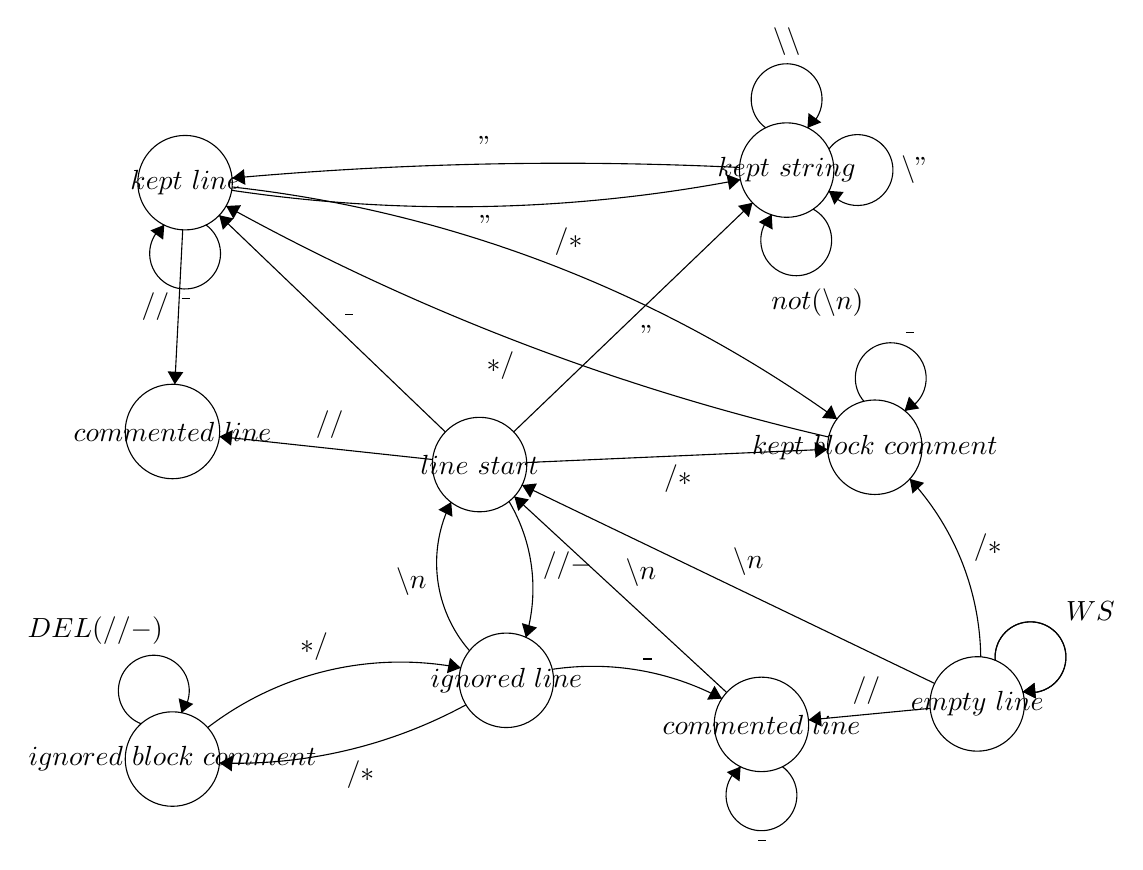
\begin{tikzpicture}[scale=0.2]
\tikzstyle{every node}+=[inner sep=0pt]
\draw [black] (32.6,-29.8) circle (3);
\draw (32.6,-29.8) node {$line\mbox{ }start$};
\draw [black] (34.3,-43.5) circle (3);
\draw (34.3,-43.5) node {$ignored\mbox{ }line$};
\draw [black] (13.1,-27.7) circle (3);
\draw (13.1,-27.7) node {$commented\mbox{ }line$};
\draw [black] (13.9,-11.9) circle (3);
\draw (13.9,-11.9) node {$kept\mbox{ }line$};
\draw [black] (52.1,-11.1) circle (3);
\draw (52.1,-11.1) node {$kept\mbox{ }string$};
\draw [black] (50.5,-46.3) circle (3);
\draw (50.5,-46.3) node {$commented\mbox{ }line$};
\draw [black] (13.1,-48.5) circle (3);
\draw (13.1,-48.5) node {$ignored\mbox{ }block\mbox{ }comment$};
\draw [black] (64.2,-45) circle (3);
\draw (64.2,-45) node {$empty\mbox{ }line$};
\draw [black] (57.7,-28.7) circle (3);
\draw (57.7,-28.7) node {$kept\mbox{ }block\mbox{ }comment$};
\draw [black] (34.467,-32.136) arc (30.72442:-16.57734:10.855);
\fill [black] (35.54,-40.78) -- (36.25,-40.15) -- (35.29,-39.87);
\draw (36.58,-36.21) node [right] {$//-$};
\draw [black] (29.62,-29.48) -- (16.08,-28.02);
\fill [black] (16.08,-28.02) -- (16.82,-28.6) -- (16.93,-27.61);
\draw (23.08,-28.16) node [above] {$//$};
\draw [black] (34.77,-27.72) -- (49.93,-13.18);
\fill [black] (49.93,-13.18) -- (49.01,-13.37) -- (49.7,-14.09);
\draw (43.28,-20.93) node [below] {$"$};
\draw [black] (30.43,-27.73) -- (16.07,-13.97);
\fill [black] (16.07,-13.97) -- (16.3,-14.89) -- (16.99,-14.17);
\draw (24.27,-20.37) node [above] {$\_$};
\draw [black] (13.75,-14.9) -- (13.25,-24.7);
\fill [black] (13.25,-24.7) -- (13.79,-23.93) -- (12.79,-23.88);
\draw (12.93,-19.78) node [left] {$//$};
\draw [black] (49.163,-11.711) arc (-79.13969:-98.46084:96.269);
\fill [black] (49.16,-11.71) -- (48.28,-11.37) -- (48.47,-12.35);
\draw (33.05,-13.93) node [below] {$"$};
\draw [black] (15.223,-14.58) arc (54:-234:2.25);
\draw (13.9,-19.15) node [below] {$\_$};
\fill [black] (12.58,-14.58) -- (11.7,-14.93) -- (12.51,-15.52);
\draw [black] (35.6,-29.67) -- (54.7,-28.83);
\fill [black] (54.7,-28.83) -- (53.88,-28.37) -- (53.93,-29.37);
\draw (45.2,-29.8) node [below] {$/*$};
\draw [black] (16.887,-12.173) arc (83.71258:54.31763:81.07);
\fill [black] (55.3,-26.91) -- (54.94,-26.03) -- (54.35,-26.84);
\draw (38.25,-16.54) node [above] {$/*$};
\draw [black] (57.014,-25.792) arc (221.00538:-66.99462:2.25);
\draw (59.88,-21.55) node [above] {$\_$};
\fill [black] (59.59,-26.39) -- (60.52,-26.24) -- (59.87,-25.48);
\draw [black] (54.771,-28.052) arc (-103.04429:-118.92551:148.313);
\fill [black] (16.51,-13.38) -- (16.97,-14.2) -- (17.45,-13.33);
\draw (33.92,-22.57) node [below] {$*/$};
\draw [black] (16.886,-11.611) arc (95.15989:87.23958:233.306);
\fill [black] (16.89,-11.61) -- (17.73,-12.04) -- (17.64,-11.04);
\draw (32.98,-10.2) node [above] {$"$};
\draw [black] (50.777,-8.42) arc (234:-54:2.25);
\draw (52.1,-3.85) node [above] {${\setminus{}}{\setminus{}}$};
\fill [black] (53.42,-8.42) -- (54.3,-8.07) -- (53.49,-7.48);
\draw [black] (54.78,-9.777) arc (144:-144:2.25);
\draw (59.35,-11.1) node [right] {${\setminus{}}"$};
\fill [black] (54.78,-12.42) -- (55.13,-13.3) -- (55.72,-12.49);
\draw [black] (53.772,-13.576) arc (61.76517:-226.23483:2.25);
\draw (54.05,-18.59) node [below] {$not({\setminus{}}n)$};
\fill [black] (51.15,-13.93) -- (50.33,-14.4) -- (51.21,-14.88);
\draw [black] (31.972,-41.632) arc (-138.85121:-207.00172:8.5);
\fill [black] (30.8,-32.18) -- (29.99,-32.67) -- (30.88,-33.12);
\draw (29.27,-37.22) node [left] {${\setminus{}}n$};
\draw [black] (37.214,-42.802) arc (98.52659:61.86122:17.383);
\fill [black] (47.99,-44.66) -- (47.52,-43.85) -- (47.05,-44.73);
\draw (43.21,-42.27) node [above] {$\_$};
\draw [black] (31.738,-45.058) arc (-61.50966:-91.94905:30.623);
\fill [black] (16.09,-48.75) -- (16.87,-49.28) -- (16.91,-48.28);
\draw (25.03,-48.55) node [below] {$/*$};
\draw [black] (48.29,-44.27) -- (34.81,-31.83);
\fill [black] (34.81,-31.83) -- (35.06,-32.74) -- (35.73,-32.01);
\draw (42.85,-37.56) node [above] {${\setminus{}}n$};
\draw [black] (51.823,-48.98) arc (54:-234:2.25);
\draw (50.5,-53.55) node [below] {$\_$};
\fill [black] (49.18,-48.98) -- (48.3,-49.33) -- (49.11,-49.92);
\draw [black] (15.334,-46.502) arc (127.53688:79.00441:20.093);
\fill [black] (31.41,-42.71) -- (30.72,-42.07) -- (30.53,-43.05);
\draw (22.09,-42.28) node [above] {$*/$};
\draw [black] (11.119,-46.263) arc (249.25512:-38.74488:2.25);
\draw (8.2,-41.25) node [above] {$DEL(//-)$};
\fill [black] (13.67,-45.57) -- (14.42,-45) -- (13.49,-44.64);
\draw [black] (65.346,-42.24) arc (185.18593:-102.81407:2.25);
\draw (69.82,-39.1) node [right] {$WS$};
\fill [black] (67.09,-44.23) -- (67.93,-44.66) -- (67.84,-43.66);
\draw [black] (65.346,-42.24) arc (185.18593:-102.81407:2.25);
\fill [black] (67.09,-44.23) -- (67.93,-44.66) -- (67.84,-43.66);
\draw [black] (59.919,-30.714) arc (42.71431:0.76725:16.992);
\fill [black] (59.92,-30.71) -- (60.09,-31.64) -- (60.83,-30.96);
\draw (63.96,-35.06) node [right] {$/*$};
\draw [black] (61.21,-45.28) -- (53.49,-46.02);
\fill [black] (53.49,-46.02) -- (54.33,-46.44) -- (54.24,-45.44);
\draw (57.17,-45.07) node [above] {$//$};
\draw [black] (61.5,-43.7) -- (35.3,-31.1);
\fill [black] (35.3,-31.1) -- (35.81,-31.9) -- (36.24,-31);
\draw (49.66,-36.89) node [above] {${\setminus{}}n$};
\end{tikzpicture}
\end{center}
\caption{Approximate finite state machine for removing redundant commenting
    from a C file.}\label{fig:comment-simp-fsm}
\end{figure*}

\section{Limitations and future work}

Further input validation on the formatting of fields \emph{within} structs and
unions is also desirable, and should be a relatively straightforward feature to
add.

A useful sanity check on the output of the tree carver is compiling the output
with the same compile command, which should and does not (for the examples we
have used it with so far) produce more warnings than the input code. It would
be even better if the output could be compiled and linked, but this is a
cross-translation-unit issue and the Clang API is fundamentally a
per-translation-unit one, so this requires more consideration and perhaps a
different approach.

Another limitation is that right now, struct fields are omitted with no
replacement, which changes their size. This should be possible to remedy, since
the size and padding of a field are available when traversing the declaration
of a struct field, but leads to a more complex `marking' scheme per line than
the binary included or not. It may also complicate any attempts to link the
code with other code that uses the same struct definitions but different
fields.

\chapter{Proof maintenance for pKVM buddy allocator}\label{chap:buddy}

\margintoc{}

The \kl{pKVM} hypervisor is intended to provide isolation between virtual
machines, protecting both the guest from the host and vice versa. It is also
intended to support creating and destroying virtual machines dynamically, and
so one of its key features it needs to implement is memory management. It
implements a buddy allocator~\sidecite{knowlton1965fast} to manage the pages it
allocates. The example is discussed in \sidetextcite{pulte2023cn}, so I will
focus only on my experience in updating the code.

\section{Successful update to intrusive free lists}

The major code change is easy to describe. The buddy allocator maintains a
doubly-linked list of free pages (per order). Initially, the pointers for these
were stored externally to the free pages, but an update to the code changed it
so that the pointers were stored intrusively, on the free pages themselves.

I found updating the proof for this to be challenging, mostly due to \kl{CN}'s
error reporting, which I will explain later, but also partly due to a lack
of experience and resulting intuition around the code and its predicates.
With significant help, I was able to make worthwhile progress on it.

The \kl{pKVM} buddy allocator is a challenging piece of code to understand and
verify. It shifts between physical and virtual addresses frequently, and I
found this difficult to follow. At the time, the original proof did not have or
use helper functions, so tracking the complex arithmetic and different `types'
(metadata, index into metadata, physical address, virtual address),
was confusing. Ownership of the pages was initially indexed by its physical
address; ownership of the metadata is indexed by a value computed from a page's
address.

On top of this, ownership for the pages is sparse, based on conditions
expressed in the metadata, hence, ownership of both are needed to perform any
operations such as coalescing two buddy pages of the same order, adding or
removing a page. In addition to the addresses computable from an index, the
free pages are also aliased via a per-order doubly-linked free list. This is
where freed pages are added, and from whence allocated pages are removed.

Aside from the mechanics of moving fields and ownership from one part of the
code to another, the update also highlighted some unhelpful assumption made in
the initial verification, which meant going back, fixing the issue, and then
redoing the efforts thus far. Although some aspects of the implementation could
be encapsulated in helper functions, and working from leaf functions up was
helpful in making worthwhile progress, eventually I hit the limits of my
cognitive capabilities and of \kl{CN}'s abstractions and error reporting.

\subsection{Carving and integrated the upstream code}
I did the update before I had a functioning tree carver, and so I had to
manually carve out and integrate the upstream changes into the pre-existing
buddy allocator proof. This was slow and tedious. It was also occasionally
error-prone, because although clang and Cerberus were helpful to sanity check
the new cutdown version, they would not complain if annotations were missing.

At the time, we did not support top-level \kl{CN} definitions in comments, and
so all the definitions (which were scattered inline, not factored out into a
separate header) made using clang difficult, since they had to be manually
commented out, and then uncommented later to use \kl{CN}.

In total, carving out and grafting the updated code took around 3 weeks.

\subsection{Deleting old fields}
I started by commenting out all the instances where struct fields had been
removed (forward/backward pointers deleted from the metadata array). I
was able to do this and verify one of the functions, `hyp\_put\_page'
in approximately 1 week.

This change was straightforward to propagate in specifications because CN
reliably showed errors where non-existent fields were accessed. It was less
clear, as someone new to the code and its invariants, what the required
adjustments to the invariants needed to be. Surprsingly, I could leave this
until later \textemdash{} the changes were close to dependency leaf nodes, and
the original design \& use of the resource and logical predicate definitions
(on the non-leaf functions) did a good job of encapsulating their details.

\subsection{Adding new fields}

After propagating the removed fields, my progress slowed significantly. The
next steps required understanding the code and \kl{CN} far more deeply, namely
understanding \textemdash{} and then writing the correct predicates for
\textemdash{} free pages with intrusive doubly-linked list pointers. Thomas
Sewell, who worked on the initial proof, wrote the first draft of the new
predicate to describe such pages. This took him about a day; the new predicate
had new output values (for the previous and next pointers), and propagating
this took me about 2 weeks. I also consulted with the Christopher Pulte, who
also worked on the inital proof, who advised on further refinements, which took
another 2 weeks to propagate.

% This change removed the use of the
% `vmemmap\_b\_wf` logical function, and constraining the indices for which
% `AllocatorPage` predicates were iterated over (for `.refcount == 0` and
% `.order != hyp\_no\_order()`). Propogating this change took about 2 weeks.

\subsection{Physical to virtual address}

During the update, an issue around resource management which was previously
obscured became clearer: the code was using virtual addresses to read the
intrusive list pointers, and thus implicitly claiming ownership of the pages
via the \emph{virtual} rather than physical addresses.

Unfortunately, the original verification claimed ownership for the pages via
the physical addresses. This was fine in the orignal proof and code, because
the pages were never read from; but it is impossible to convince \kl{CN} that
loading a struct from a virtual address whilst it has ownership of the
distantly related physical one, since that would collapse the distinction and
transformations between them.

The remedy to this was to go back and update the original proof to consistently
use ownership via virtual addresses, in anticipation of the forthcoming
changes. Fixing and then propogating these changes, alongside cosmetic changes,
in the rebase took one month.

\subsection{Helper functions}

After the rebase, I verified two new helper functions. The first of these takes
a pointer to a free page's metadata, converts it into the virtual address for
the free page itself, and then deletes the page from the doubly-linked free
list it is in. The second is similar, but adds the page to a specified
double-linked free list.

Their specifications were verbose, but not too challenging \textemdash{} the
standard list functions they wrapped up were already verified in the previous
proof, so it was a matter of plumbing through enough invariants to support
computing the virtual address (and associated ownership) from a page metadata
pointer.

For verification, it was useful to add an extra wrapper around each these
helper functions, which expressed the addition/removal in higher-level
invariants used by the main functions. To express those invariants, the
verification helpers needed an extra logical parameter, but since
\kl{CN} does not currently support those (when not derived from program
variables), the parameter was reified into the C code (but ignored in the
body).

\subsection{Indexing and signed bit vector division}

The main predicate of the buddy allocator claims a contiguous iterated
ownership of page metadata, and \emph{spare} iterated ownership of the pages
themselves, specifically the free pages (determined by the metadata).

As I mentioned before, the code assumes that it can dereference the contents of
pages via their \emph{virtual} addresses. So this gives two seemingly equally
valid choices on how to \emph{index} the iteration that iteration. It could
either be indexed according to the same scheme as the metadata, or it could be
indexed by a \emph{virtual index}. The latter is more natural to write, since
the base virtual index is always 0, and the base virtual address is always 0,
and was the initial choice for expressing this.

However, this quickly became unwieldy as logical expressions using the
\emph{outputs} of these differently indexed arrays need to convert between the
two consistently and correctly. Not only was this not the case, lurking beneath
the conversion was a division of a signed bit vector in Z3, which folklore
suggests is ill-advised for performance.\sidenote{I thank Thomas Sewell for
alerting me to this; though in this instance, it is not clear this was the
bottleneck.} Hence, the penultimate step to verifying the code was
standardising these indices and avoiding the possibility of signed bit vector
division, which took about 1 week.

\begin{figure}[tp]
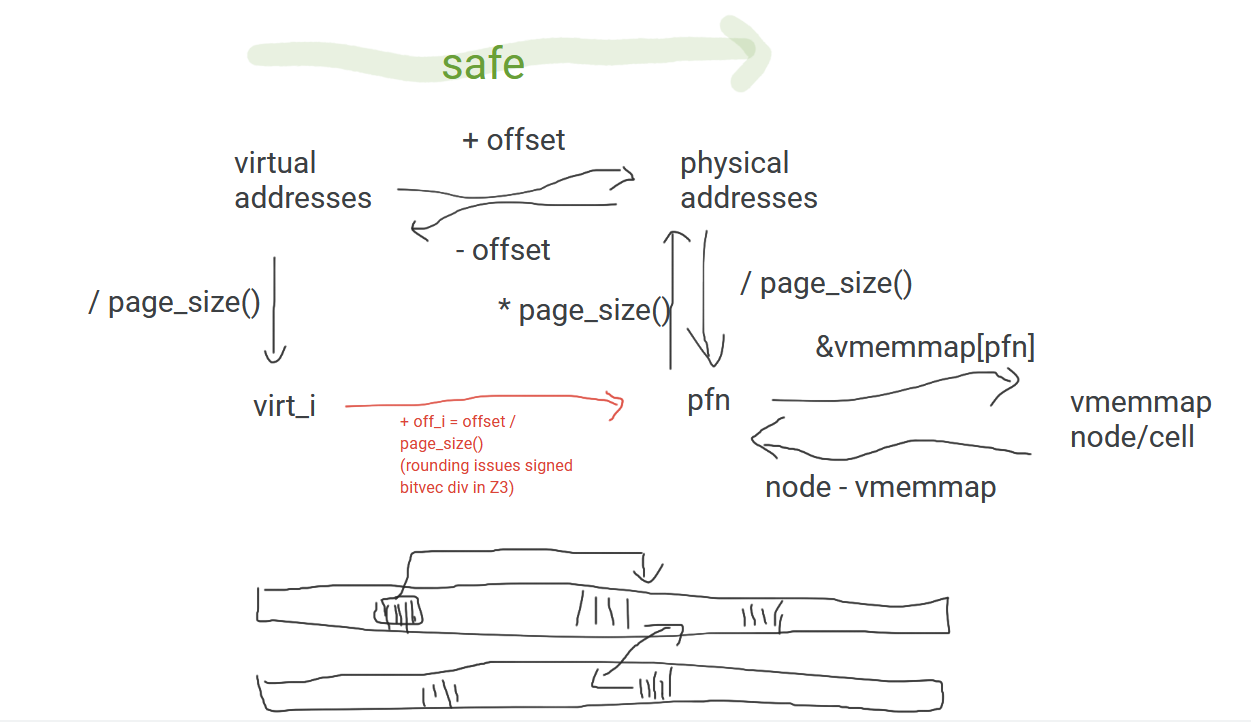
\includegraphics{figures/buddy-negative-div.png}
\caption{Negative divisions causing potential issues.}\label{fig:buddy-negative-div}
\end{figure}

\subsection{Stuck in complexity}

After I had finished verifying the leaf and the intermediate functions, I
became stuck because of the sheer complexity and unfamiliarity of the top-level
predicate, as well as usability issues I will cover soon.\sidenote{I had also
started work on the tree carver, which was much more tractable/appealing.}

Thomas Sewell took over and completed the updated proofs at this stage. The key
insight to enable this was the realisation that the main invariant needed to
variants such that zero, one or two pages could be removed from it, but
otherwise still hold, so that the ownership of a page and its buddy could be
removed, coalesced, and returned in a way that preserved the original structure
of the code, which took at most 2 weeks.

\section{Successful update to experimental VIP}

Towards the end of the update to support the intrusive free lists, I started
working up updating the buddy allocator proof to an early version of the
\kl{VIP} implementation. In this early version, pointers were augmented with an
allocation ID, and the typing rules were updated to handle this. I had
implemented a flag for turning \kl{VIP} behaviour on and off, and also
non-deterministic pointer equality; I had yet to implement a separate
\cinline{NULL} constructor in the SMT representation of pointers, or pointer
liveness and bounds checks.

The modifications I made concerned only integer-to-pointer casts:
\begin{itemize}
    \item Changed all integer-to-pointer casts in the specifications to use,
        array or member shifting, or \cinline{copy_alloc_id}.
    \item Changed the pointer to the base of the metadata array from an integer
        to a pointer.
        %\cinline{u64 __hyp_vmemmap} to \cinline{struct hyp_page *__hyp_vmemmap}.
        In the absence of support for round-trip casts, this small change gave
        the frequently used pointer a valid allocation ID\@.
    \item Changed 5 instances of a \emph{computed} integer to pointer cast to
        to use \cinline{copy_alloc_id}. I added a new global pointer to
        to indicate which allocation the new pointers should all belong to.
\end{itemize}

Given the pervasiveness of computed pointers in the code and specifications,
the changes were extensive but straightforward. The updated proof was backwards
compatible: it passed both with and without the early \kl{VIP} rules enabled.

\section{Failed update to support bit vectors}\label{sec:buddy-failed-bv}

The \kl{VIP} update was intentionally small and early, so that I could iterate
on it frequently and incrementally, whilst keeping the hero example of \kl{CN}
functional at each step.

This did not pan out due to a substantial change to \kl{CN}: switching the
representation of integers from mathematical integers to fixed-width bit
vectors. In short, the change made verifying the buddy allocator at at least
50x slower, and, remarkably, this went unnoticed for a long time. The reasons
for this will become clear in the following takeaways.

\section{Key takeaways}

% Some list functions were given more general specifications, in particular, the
% remove functions now support "removal" from a self-cyclic list, which amounts
% to a no-op. d0a4c2a15557038948f4678d29e0d529d33caa00

\subsection{Features}\label{subesc:takeaway-features}

\paragraph{Tutorials are indispensable.} The buddy allocator verification is
complex, and learning it without building up intuition for separation logic and
how to operate \kl{CN} made the process unnecessarily difficult. This has been
remedied with the introduction of the \kl{CN
tutorial}.\sidecite{pulte2024tutorial}

\paragraph{Tree carving is indispensable.} Manually carving and grafting the
code took a significant amount of time (3 weeks), once again demonstrating the
need and usefulness of the tree carver as an integral part of any usable C
verification tool.

\paragraph{Functions should be checked in dependency order.} From the get go,
the default order in which \kl{CN} checked its functions was unhelpful.
Ideally, one would like it to start with leaf functions and then work its way
up, but instead the user must figure out and maintain the dependency structure
in their head when planning the proof effort, and manually select the functions
to verify one at a time.

\paragraph{Function-like macros represent real abstractions.} The buddy allocator code
uses function-like macros heavily to convert between a pointer to metadata, an
index into metadata, a physical address and a virtual address. Ideally there
would be some way of automatically converting such macros into logical (ghost)
functions, but this is difficult because macros can and do refer to global
variables. Instead of converting macros to logical functions, it may be more
fruitful to simply expand their use in specifications, but macros are not
expanded in comments, where \kl{CN}'s annotations live.\sidenote{This is close
to essential for maintaining compatibility with existing C tool chains.}
\kl{CN} does have an experimental feature for lifting a C function into a
logical one, with the idea being that writing a C function around a macro call
is an option sometimes. All this being said, even if by hand, the benefit of
defining logical equivalents of function-like macros is worthwhile for the
readability, reliability and maintainability it brings.

\paragraph{Constant-like macros also represent real abstractions.} I spent a
bit of time removing magic constants prevalent in the original proof. Part of
this was just human inconsistency, part of this was two syntactic limitations
of an earlier version of \kl{CN}. The first was that in that in top-level
definitions, one could write \cninline{sizeof<struct hyp_page>}, but not in the
specifications. The second was that step sizes in iterated predicates must be
integer literals (rather than \cninline{sizeof<>} expressions). This was
exacerbated by the fact that the size of \cinline{struct hyp_page} shrank
between the versions from 32 to 4, and the size of its \cinline{.order} field
shrank from \cinline{u32} to \cinline{u8}. Correspondingly, the constant
\cinline{HYP_NO_ORDER} shrank from \cinline{UINT_MAX} (4294967295) to 255. All
of these required several tedious updates to the code when a well-placed
abstraction would have served well.

\paragraph{Multiple specifications/wrapper functions in annotations are
necessary.} Adding wrapper functions is useful to break down the problem of
relating complex global invariants down to more local ones required for
manipulating fundamental data-structures. Whilst this was a useful verification
strategy, to upstream such code would require the verification-only C functions
to be removed, and replaced with annotation-only mechanisms.

\paragraph{But also, allow wrapper functions to be inlined.} Requiring
specifications for all top-level functions is useful in theory, but actually
increases the cost of using them when verifying code. Allowing functions to be
verified by inlining at call site, rather than by specification, would
alleviate this, although of course, this would be open to abuse too.

\paragraph{Explicit ghost parameters and arguments are necessary.} Changing the
C code by adding unused parameters to support proof would not be acceptable in
almost all large, real-world code bases. Reifying ghost parameters complicates
specifications in tangible ways too: Adding a page to the free list requires
converting a metadata pointer into a virtual address, and doing so requires
appropriate range constraints. Without ghost parameters and arguments, the only
way to get the values for those constraints is to pass in ownership of a struct
containing them (and then constrain that the value has not changed, which is
easy to forget and painful to debug). However, the same struct also contains
ownership of the per-order free list array, which contains the \emph{other}
parameter of the function. Using that parameter requires ownership, and so if
one is not careful, naively adding an extra parameter can lead to a claiming
ownership of the same location twice.\sidenote{See
\href{https://github.com/rems-project/cn-pKVM-buddy-allocator-case-study/commit/3363734d706a90a4674c44fa36dd0babcf93b084}{commit
3363734}.} Spotting this error requires some deep familiarity with \kl{CN}.
Hence, all of this would be avoidable if ghost arguments could be passed
directly.

\paragraph{Globals should be implicitly in scope and read-only.} Forgetting the
`\cninline|{_} unchanged|' annotation in a specification leads to spurious
errors between calls to functions which use `\cninline{accesses _}' on the same
globals in their specifications.

\paragraph{Syntax needs to support `overriding' invariants.} The main invariant
on the allocation pool of the hypervisor is sometimes broken at one or two
indexes, and there is no simple way to express this in the current syntax. This
not only causes duplication of top-level predicates, but it also causes many
conditions to be inlined into annotations, such as loop invariants, making them
less readable and less understandable.

\subsection{Handling large changes}\label{subsec:handling-large-changes}

\paragraph{Substantial changes should be opt-in/gated underneath a flag.}
\kl{CN}'s transition to bit vectors was to support reasoning about \kl{pKVM}'s
page table code, which used bit manipulation extensively, without resorting to
lemmas frequently. However, the change was compulsory, rather than optional,
and it left updating the buddy allocator high and dry, rather than turned on
after understanding the specification and performance overhead.

\paragraph{Syntax changes should be opt-in/gated underneath a flag.} The update
to bit vectors changed the syntax of integer types too, and this was tedious to
update manually. Either refactoring tools for specifications need to be
developed to assist with this, or changes need to be brought in less abruptly.

\paragraph{Constraints on bit vectors should exclude overflow.} With integers,
it is possible to constraint $a$ by constraining $a \times{} 4096$, with bit
vectors, it is not. Thus, by default, specifications on bit vectors parameters
(including addresses of pointers) need to be phrased in terms of the original
variables rather than on subsequent expressions which could overflow. This also
hints a relatively simple scheme for translating specifications on integers
into bit vectors.\sidenote{Refinement types for refinement types.}

\subsection{Error messages}

\paragraph{Accurate source location information is paramount, especially in the
presence of elaboration and auto-generated variables.} Though \kl{Cerberus}'
elaboration is compositional, this does not mean the accurate and helpful error
messages come for free. For example, it is very helpful to relate source
location of generated variables to that of the expressions they are
binding.\sidenote{\href{https://github.com/rems-project/cerberus/issues/270}{Cerberus
\#270}.} Aside from that, in earlier versions of \kl{CN}, the main datatype
for representing SMT terms did not carry source location information. Which
made it very difficult to track down which part of a pre- or postcondition was
failing, or which subterm in a large expression was not well-formed. This also
fed into making counter-examples much less useful.

\paragraph{Aliasing, and conditionally aliasing variables need to be presented
clearly.} For example, the list manipulation functions take arguments which may
alias each other, and the ownership in both cases is quite different.
Understanding which case one is in, and how the two different aliases relate
can get confusing.
% Any situation where memory is "split" into logical operations gets confusing.
% For instance, in the return contracts of the list functions, which have
% input/ouput values "Owned(next) if next != prev", *next doesn't mean what you
% might think, with the C *next being (next == prev ? *prev : *next) in CN.

\paragraph{Counter-examples should be related to what the user wrote.} CN's
presentation of counter-example models was and remains unhelpful, though
improvements to the naming scheme for automatically generated variables, and
outputting sub-terms as well as top-level failed constraints, did blunt the
impact slightly. Whilst I changed the debug printing of index terms in failed
constraints to annotate sub-terms with their values, and indent them properly,
the best solution would be to annotate the original source with the
counter-example model values.

\paragraph{Counter-examples should be minimal and consistent.} Another source
of confusion is that counter-examples are neither minimal, nor consistent: all
variables are assigned a value, values irrelevant to counter-example may not be
consistent with the constraints, and it is not possible to query the solve to
determine which variables are relevant, and which may be safely ignored.

\paragraph{Counter-examples should be easy to understand.} Values in
counter-examples can be quite large and thus difficult to parser and check
mentally. A trick I learned from Thomas Sewell was to add requirements to a
function failing to verify which assert that, for instance, the
physical/virtual offset is 0 and the pool is limited to a tiny range of small
memory addresses. Constraining values to be small reduces makes
counter-examples more manageable, and this should be automated.

\paragraph{Counter-examples should be interactive.} With small values, minimal
models and good relatability to the source, it should be possible to make
counter-examples interactive, such as stepping through the program, or tracing
out the shape of the symbolic heap (ideally graphically) to make it much easier
to visualise where a user's intuitions and assumption do not match the code's.

\paragraph{Counter-examples with iterated resources and quantified constraints
need special care.} In particular, it it is tricky to debug
inconsistent/incorrect indexing across different terms.

